\documentclass[11pt]{article} % For LaTeX2e
\usepackage{manuscript, palatino}
\usepackage{graphicx}
\usepackage{amsfonts, amsmath}
\usepackage{algorithm, algpseudocode}%

\usepackage{natbib}

\title{Anxiety: a decision-theoretic perspective}

\author{
Samuel Zorowitz \\
Princeton Neuroscience Institute\\
Princeton University\\
Princeton, NJ 08540 \\
\texttt{zorowitz@princeton.edu} \\
\And
Ida Momennejad \\
columbia University\\
New York, NY 10027 \\
\texttt{ida.m@columbia.edu} \\
\And
Nathaniel Daw \\
Princeton Neuroscience Institute\\
Princeton University\\
Princeton, NJ 08540 \\
\texttt{ndaw@princeton.edu} \\
}

\newcommand{\fix}{\marginpar{FIX}}
\newcommand{\new}{\marginpar{NEW}}

\begin{document}

\maketitle

\begin{abstract}
To be filled in
\end{abstract}

\keywords{
reinforcement learning; avoidance; anxiety
}

\startmain

\section{Introduction}
Many psychiatric disorders involve distortions in models of the external world
and, correspondingly, aberrations of learning and decision making. As a normative
framework, decision theory allows us to describe and pose quantita­tive questions
about optimal and approximately optimal choice behavior \citep{DayanDaw2008} and
is, therefore, a critical tool for modeling, understanding, and predicting the
psychological and neurobiological mechanisms responsible for the abnormalities
observed in psychiatric behavior \citep{HuysDawDayan2015}. Many recent investigations
employing this approach have provided important insights into psychiatric symptoms,
including anhedonia in major depression \citep{Rutledge2017}, mood instability
in bipolar disorder \citep{EldarNiv2015, EldarDolanNiv2016},  habitual decision
making in disorders of compulsivity \citep{gillan2016}, and hallucinations in
schizophrenia \citep{powers2017, corlett2018}.

Anxiety disorders (generalized anxiety disorder, social anxiety disorder, panic
disorder, obsessive-compulsive disorder) represent the most common family of
psychiatric disorders (citation). Despite the differences in the content of worry,
all anxiety disorders share two core features: pessimistic inference and excessive
avoidance. Pessimistic inference describes a tendency to appraise threatening
situations as more frequent and/or more severe than they objectively are. This has
been reliably observed experimentally, as in fear conditioning wherein individuals
with anxiety exhibit exaggerated fear towards safe cues (CS-) and extinguished
threatening cues \citep{lissek2005, Duits2015}, and clinically, through self-report
(pick 3 citaitons). Excessive avoidance describes the corresponding tendency for
individuals with anxiety to consistently flee or avoid threatening situations.
Avoidance is often chosen even at the expense of potential reward (approch-avoidance
conflict), and is frequently a major impediment to recovery \citep{Arnaudova2017}.

Recent studies have attempted to provide some computational models of this behavior
\citep{Moutoussis2008, Maia2010}. For example, \citep{Maia2010} was able to show
how reinforcement learning could explain sustained avoidance in the absence of
repeated reinforcement, observed in rodents \citep{servatius2008} and something
not explained by two-factor theory \citep{Krypotos2015}. As has been discussed
elsewhere \citep{Moutoussis2017}, such accounts only explain the maintenance of
avoidance in short timescales, but do not explain why resistant to change and
why they do not go away in general. Such theories also do not explain the magnitude
of pessimistic inference, or the fear generalization. A broader account is needed.

In this article, we put forward a decision theoretic explanation of the core
symptoms of anxiety. In sequential decision environments, we show how a loss of
optimistic inference results in pessimistic inference, chronic avoidance, and
generalization of fear.

\section{Methods}

\subsection{Markov Decision Processes}

Here, we briefly review the formalism of Markov decision processes (MDPs), which
provide the foundation for our results. For more complete treatments of the
subject, see Sutton \& Barto (1998, 2018) and Bertsekas \& Tsitsiklis (1996).

A MDP is defined by a set of states, $S$, a set of actions, $A$, a reward
function, $R(s,a)$ over state/action pairs, and a state transition distribution,
$P(s'|s,a)$, where $a$ denotes a chosen action. States and rewards occur
sequentially according to these one-step functions, driven by a series of
actions; the goal is to learn to choose a probabilistic policy over actions,
denoted by $\pi$, that maximizes the value function, $V^\pi(s)$, defined as the
expected cumulative discounted reward:

$$ V^\pi(s) = \mathbb{E} \left[ \sum^{\infty}_{k=0} \gamma^k R_{t+k} | S_t = s \right] $$

Here, $\gamma$ is a parameter controlling temporal discounting. The value function
can also be defined recursively as the sum of the immediate reward of the action
chosen in that state, $R(s, a)$, and the value of its successor state $s’$,
averaged over possible actions, $a$, and transitions that would occur if the agent
chose according to $\pi$:

$$ V^\pi(s) = \sum_a \pi(a|s) \left[ R(s,a) + \sum_{s'} P(s'|s,a) \gamma V^\pi (S') \right] $$

The value function under the optimal policy is given by:

$$ V^*(s) = \max_a \mathbb{E} \left[ \sum^{\infty}_{k=0} \gamma^k R_{t+k} | S_t = s \right] $$

$$ = \max_a \left[ R(s,a) + \sum_{s'} P(s'|s,a) \gamma V^\pi (S') \right] $$

Knowledge of the value function can help to guide choices. For instance, we can
define the state-action value function as the value of choosing action $a$ and
following $\pi$ thereafter:

$$ Q^\pi(s,a) = \mathbb{E} \left[ \sum^{\infty}_{k=0} \gamma^k R_{t+k} | S_t = s \right] $$

$$ = R(s,a) + \sum_{s'} P(s'|s,a) \gamma V^\pi (S') $$

Then at any state one could choose the action that maximizes $Q^\pi(s,a)$. Formally
this defines a new policy, which is as good or better than the baseline policy
$\pi$; analogously, Eq 2 can be used to define the optimal state-action value
function, the maximization of which selects optimal actions. Note that it is
possible to write a recursive definition for $Q$ in the same manner as Eq 1, and
work directly with the state-action values, rather than deriving them indirectly
from $V$.

\subsection{Robust Control}

To create the symptoms of anxiety, we need a loss of control. This can come in
two forms. First is through the state transition distribution, $P(s'|s,a)$.
Normally, we assume the world is deterministic; in other words, an agent's chosen
action, $a$ leads the agent to the desired successor state, $s'$. In a stochastic
environment, however, an agent may instead transition to an undesired state, $s^*$.

Importantly, in the clinical literature, pathological anxiety is also associated
with a lack of perceived control (Gallagher et al., 2014). Studies suggest that
this belief mediates anxiety (ref?). This can come in whatever form.

Alternately, an agent may choose optimally in the present but may be uncertain of
its choice control in the future. In such a case, we deviate from the optimal
policy in the future. We can adopt a different function. There are a number to
choose from \citep{Garcia2015}. Here we adopt the beta-pessimism criterion
\citep{Gaskett2003}:

$$ V(s') = \beta \max_{a'} Q(s',a') + (1 - \beta) \min_{a'} Q(s',a') $$

where $\beta$ controls the degree of pessimism. When $\beta = 1$, an agent expects
complete control to choose the best action (best-case criterion); when $\beta = 0$,
an agent expects the  worst future case; and when $\beta = 0.5$, an agent expects
randomness. (We are not committed to this particular instantiation; it is simply
a convenient notation. Other parameterizations work equally well, see appendix.)

\subsection{Simulations}

In some instances, we solve for Q-values and state values directly through value
iteration. This is a form of Dynamic Programming. In other instances, we estimate
these terms through temporal difference learning. We use beta-pessimism (betamax)
learning for both. We use the former to solve for final (infinite horizon) values
and the latter to identify finite horizon values. We explain when we use both.

\section{Results}

\subsection{Pessimistic Inference}

One symptom central to all of the anxiety disorders is pessimistic inference,
or a tendency to appraise the likelihood and/or severity of threatening situations
out of proportion to their actual environmental contingencies \citep{dsm5, BeckClark1997,
ClarkBeck2011}. For example, an individual with specific phobia may vastly exaggerate
the probability of encountering their fear (e.g. a venomous spider) in their
everyday lives. The first studies of pessimistic inference in clinically anxious
populations involved individuals judging the perceived likelihood and severity
of different aversive situations, with the general finding that anxious individuals
rated these as more likely than non-clinical individuals \citep{ButlerMathews1983,
ButlerMathews1987, Foa1996, MacLeod1996, MacLeod1997, Luten1997, Stober1997,
Borkovec1999}; a finding that has been replicated more recently \citep{Maner2006,
Mitte2007, Miranda2007}.

Experimentally, aberrations in threat appraisal have been repeatedly observed
in a litany of associative learning studies. Common to all of these studies,
participants learn that a particular stimulus (CS+) predicts the occurrence
of a negative outcome (e.g. shock, loud noise, aversive image). In simple conditioning,
there is some evidence to suggest that individuals with anxiety exhibit elevated
levels of response to threatening stimuli \citep{lissek2005, MinekaOehlberg2008,
Duits2015}. Importantly, conditioning studies also suggest impaired safety learning
in anxiety, wherein a stimulus never paired with an aversive outcome (CS-) is also
feared \citep{Duits2015}. Other notable findings include impaired blocking,
conditioned discrimination (AX+/BX-) (citations), and conditioned inhibition
(A+, AB-) (citations).

% I think when you come back to edit this, you need to highlight these findings
% more in the context of what you are about to explain. Pessimistic inference
% is both making bad things worse and, most importantly, that non-bad things
% become bad. Although one question is how much to include the other less
% studied paradigms

\begin{figure}
  \centerline{%
    \resizebox{1.0\textwidth}{!}{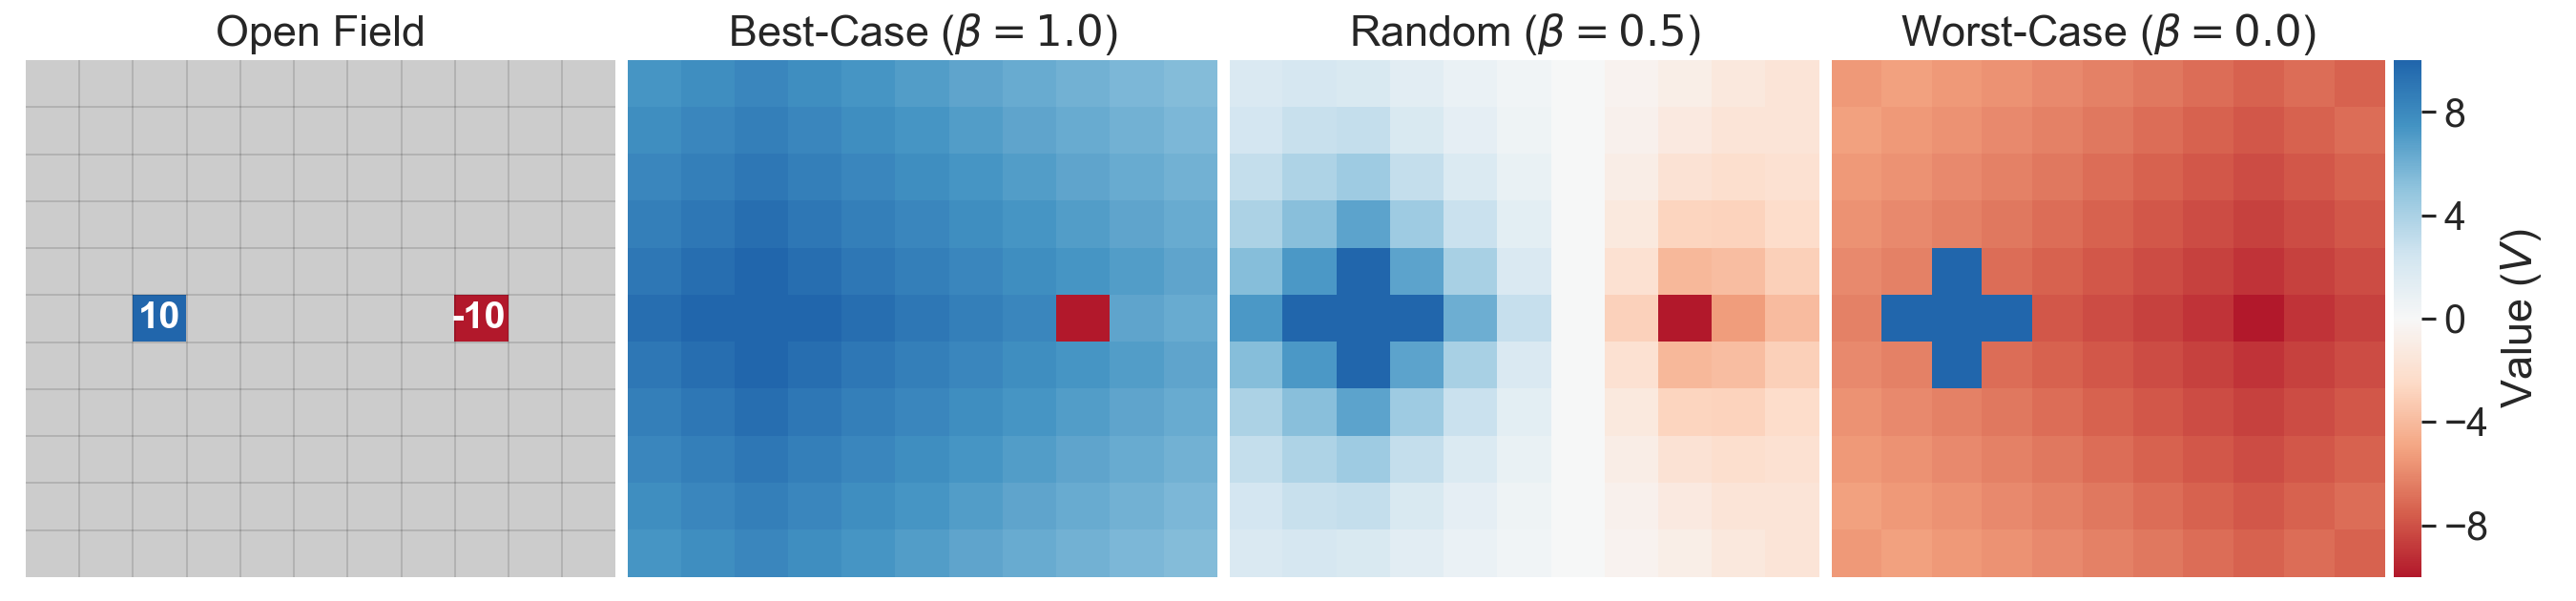
\includegraphics[trim={0 0 0 0},clip]{../figures/01_field.png}}%
  }
  \caption{\textbf{Open Field}}
  \par Current parameters: Reward = 10, Shock = -10, gamma = 0.95.
\end{figure}

In our first result, we demonstrate one simple mechanism by which pessimistic
inference and exaggerated threat appraisals may arise. In the *open field* environment,
an agent is placed in a large grid world entirely empty except for two states,
leading to positive and negative outcomes, respectively. Under complete control
(objective or perceived), an agent in this environment in under no threat despite
the presence of negative states. This is simply because, in a fully controllable
world, an agent need not ever interact with the aversive state. In fact, an agent
can decide to walk straight up to the aversive state and, insofar it does not
choose to take one step further, will never be in any actual danger.

This is not so when deterministic control cannot be assumed. If an agent believes
it is not in full control of its environment, then it cannot rule out the possibility
that it may inadvertently encounter the negative state at some point in the future,
especially if it veers to close to the state. This is true irrespective of whether
the agent believes it cannot guarantee its own future competency or the benevolence
of the environment. Importantly, this belief need not match the true environmental
statistics; belief is enough.

The long-run state values under different beliefs are plotted in Figure 1. As
expected, under optimistic beliefs (Figure 1b) the entire environment sans negative
state takes on a positive value (close to the positive state itself). As this belief
breaks down, we observe a different pattern in the long-run state values. When
future occupancy of the negative state becomes a non-zero probability, the undesired
action transition exerts influence on action-outcome calculations, back-propagating,
and thereby infecting antecedent states. As the agent's belief becomes increasingly
pessimistic, the more the worst possible action exerts influence and the more
negative, on average, the state-space grows.

In the breakdown of perceived control then, negative states can grow worse (i.e.
more predictive of future negative outcome) and otherwise positive states can too.
This occurs as a simple result that if control not guaranteed, cannot guaranteed
bad things wont happen.

% I think you want to explain second order conditioning in PTSD in this context.

\subsection{Avoidance}

A second symptom central to all anxiety disorders is avoidance \citep{dsm5,
Krypotos2015, Arnaudova2017}, or actions taken to increase or maintain the temporal,
physical and/or mental distance between an individual and a threatening situation.
Although avoidance is a natural response to danger, excessive avoidance as is
observed in anxiety disorders is can be highly disruptive to everyday functioning
\cite{Salter2004} and may work to sustain anxious appraisals and behavior. For
example, an individual with social anxiety may avoid attending large social events
for fear of public embarrassment only to never learn that such worry is not justified.

In the laboratory, avoidance has been measured in a variety of ways. In animal
models of anxiety, anxious rodents are found to exhibit avoidance learning more
quickly and maintain avoidance for longer \citep{servatius2008}. In studies of
human avoidance, anxiety has been found to correlate with the maintenance of
increased distance from threat, such as virtual predators \citep{Bach2014, Bach2017,
Sheynin2014}.

% Arnaudova2017 makes reference to some spider approach studies that might be
% interesting to try and track down. Essential idea is that even though
% participants are totally safe, may not touch the glass. The task is the
% behavioral avoidance task. (e.g. Siegel & Weinberger, 2012, emotion).
% the nice part about this is that participants are objectively safe.

There is a long history of models attempting to explain avoidance learning. The
fundamental challenge is explaining how an action can be reinforced in the
absence of an outcome. Two-factor theory was the explanation for a long while,
but suffered from a number of noteworthy criticisms \citep{Krypotos2015}.
Recent work has revitalized two-factor theory and integrated it with reinforcement
learning \citep{Moutoussis2008, Maia2010}, and in the process addressing several
criticisms of two-factor theory. As has been discussed elsewhere \citep{Moutoussis2017},
such accounts only explain the maintenance of avoidance in short timescales, but
do not explain why resistant to change and why they do not go away in general.

% Need to go into more detail than this, need to actually make this a coherent
% explanation, but this can wait for now.

\begin{figure}
  \centerline{%
    \resizebox{1.0\textwidth}{!}{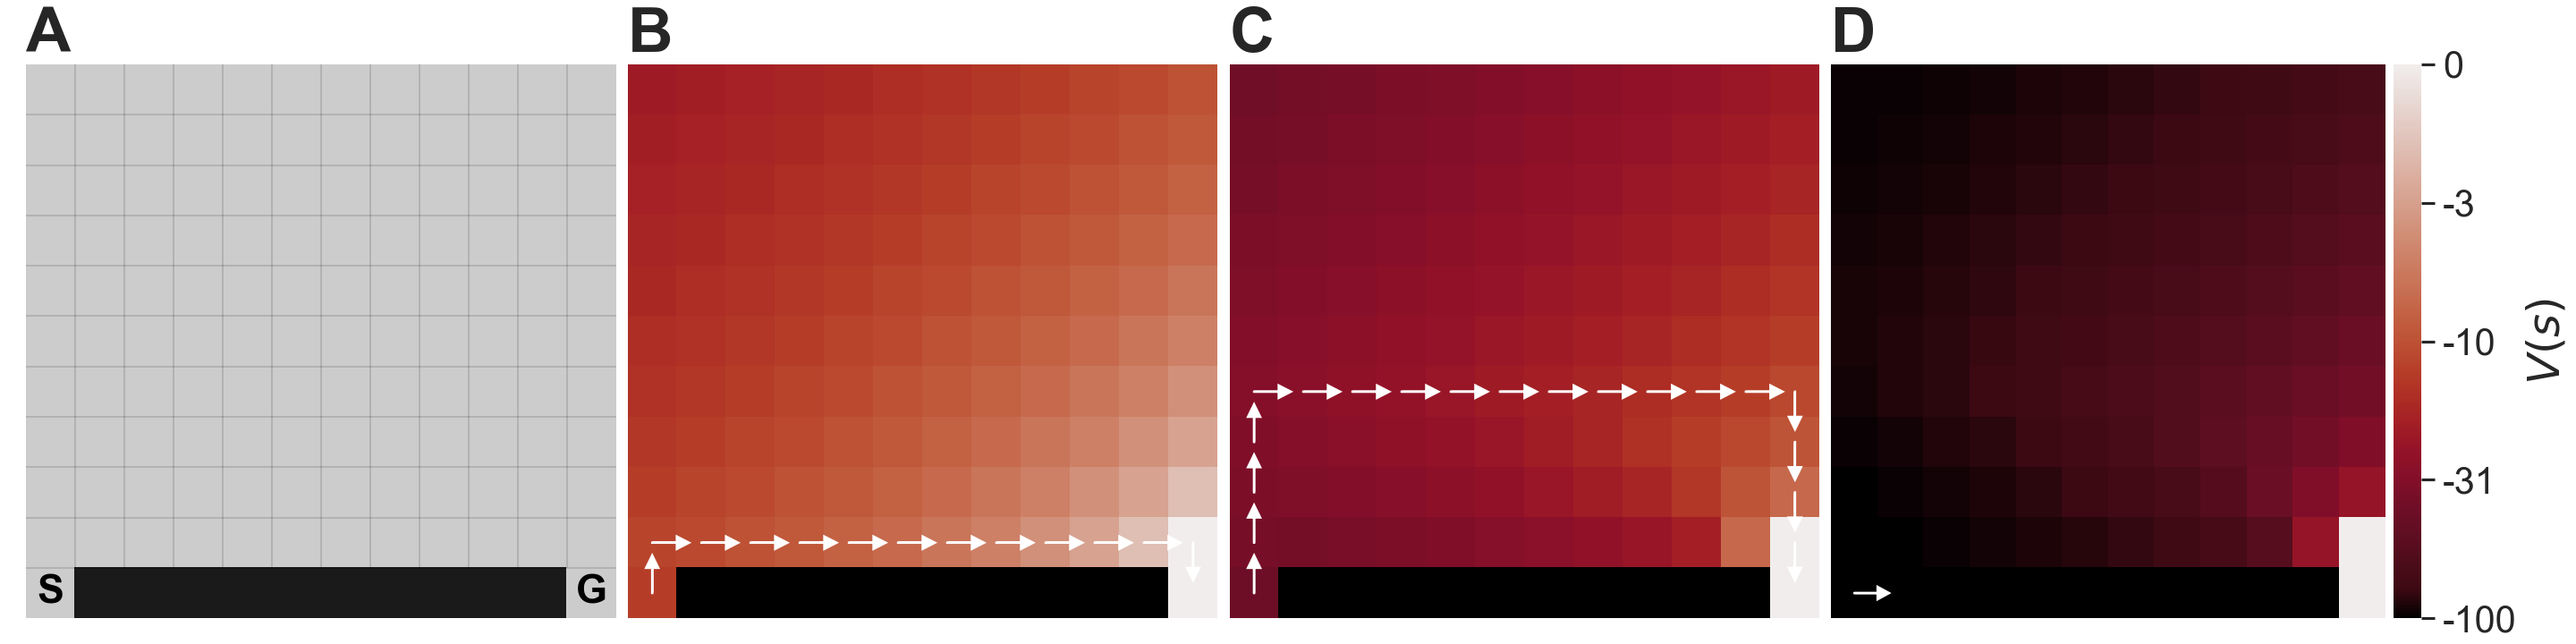
\includegraphics[trim={0 0 0 0},clip]{../figures/02_cliff.png}}%
  }
  \caption{\textbf{Cliff Walking}}
  \par Cliff = -100, Cost = -1, gamma = 0.99
\end{figure}

In our second result, we demonstrate how a breakdown in control can lead to
sustained policies of avoidance. We do so in the cliff-walking environment
\citep{SuttonBarto1998, SuttonBarto2018, Gaskett2003}. Here an agent learns to navigate from
an initial starting position to an end state. The shortest distance is along a
cliff edge. If the agent steps off the cliff, it incurs a large penalty. Under
complete control (objective or perceived), agent in this environment is under no
threat despite the presence of the cliff's edge. As in the first simulation, this
is simply because, in a fully controllable world, an agent need not ever interact
with the aversive state. In fact, an agent can decide to walk straight up to the
aversive state and, insofar it does not choose to take one step further, will
never be in any actual danger.

This is not so when deterministic control cannot be assumed. If an agent believes
it is not in full control of its environment, then it cannot rule out the possibility
that it may inadvertently encounter the negative state at some point in the future,
especially if it veers to close to the state. This is true irrespective of whether
the agent believes it cannot guarantee its own future competency or the benevolence
of the environment. Importantly, this belief need not match the true environmental
statistics; belief is enough.

The long-run state values under different beliefs are plotted in Figure 2. As
expected, under optimistic beliefs (Figure 1b) the entire environment sans negative
state takes on a positive value (close to the positive state itself). As this belief
breaks down, we observe a different pattern in the long-run state values. When
future occupancy of the negative state becomes a non-zero probability, the undesired
action transition exerts influence on action-outcome calculations, back-propagating,
and thereby infecting antecedent states. As the agent's belief becomes increasingly
pessimistic, the more the worst possible action exerts influence and the more
negative, on average, the state-space grows. Most importantly, because these are
the long-run state values, the policy is the optimal policy; in other words, this
is the long-run policy an agent will take.

\subsection{Approach-Avoidance Conflict}

Next, we turn our attention towards a related phenomenon: a bias towards avoidance
in approach-avoidance conflict. In environments with correlated risk and rewards,
a bias towards avoidance can ultimately result in fewer expected rewards and worse
long-run returns. Returning to the example above, an individual with social anxiety
may forgo social situations to avoid the risk of social embarrassment at the expense
of friendships, etc. This is another way in which pathological anxiety can be
disruptive to everyday functioning.

Experimentally, there is a long history of measuring behavior during
approach-avoidance conflict in individuals with anxiety (citation, maybe yin-yang anxiety paper).
One popular paradigm is the balloon analog risk task (BART) \citep{Lejuez2002},
which has been shown to correlate with anxiety \cite{Maner2007, Giorgetta2012}.
In the task, a participant pumps a balloon with air. For each pump, the participant
earns points. If she pumps too much, the balloon pops and she loses all points.
The participant must decide within each episode when to stop pumping. Leave time
is the measure of behavior, with earlier leave times in anxiety suggesting a
greater tendency towards avoidance.

\begin{figure}
  \centerline{%
    \resizebox{1.0\textwidth}{!}{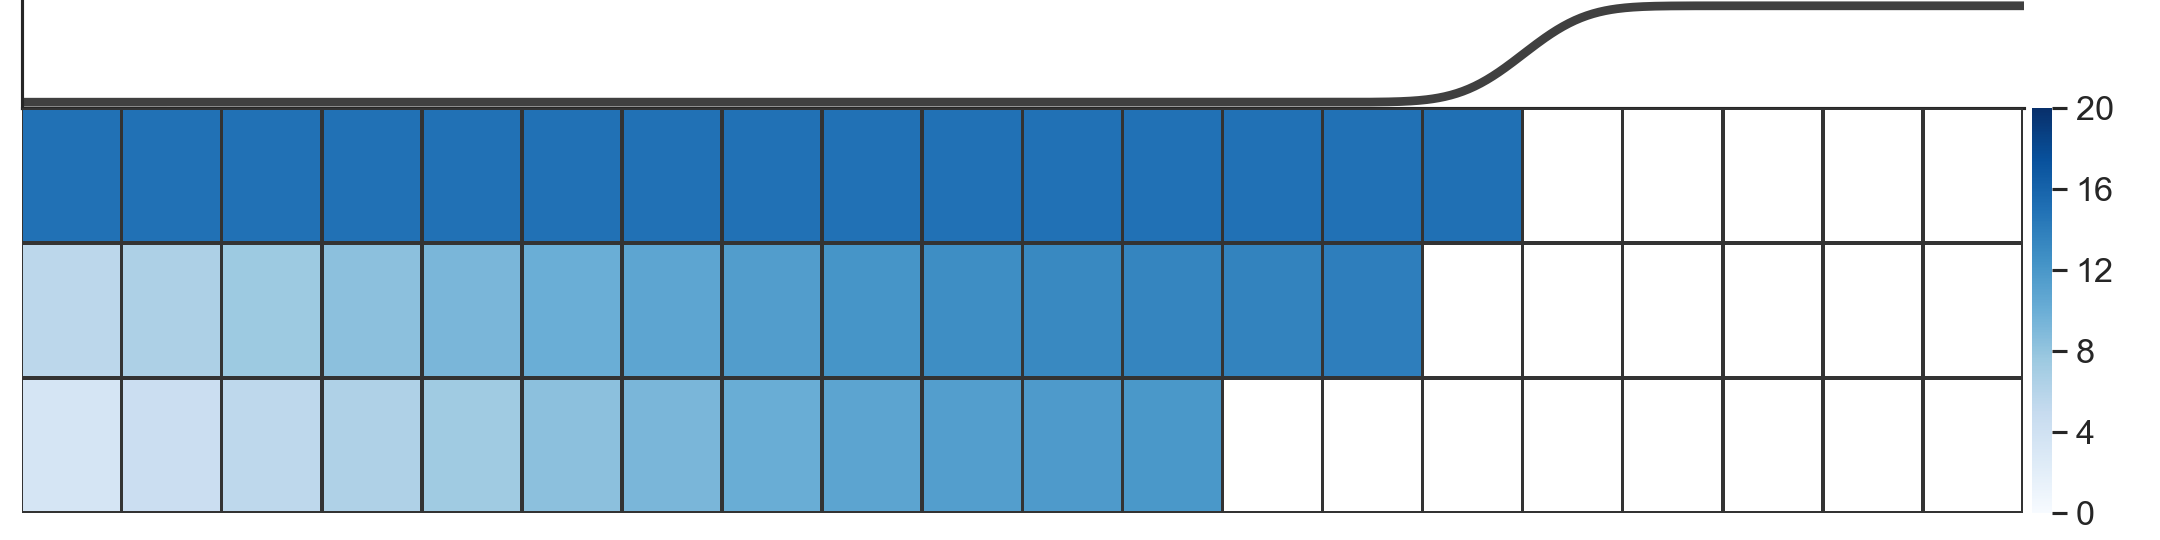
\includegraphics[trim={0 0 0 0},clip]{../figures/03_fid.png}}%
  }
  \caption{\textbf{BART}}
  \par remember to add parameters
\end{figure}

Our sequential model of decision making easily explains these results. A schematic
of the task is presented in Figure 3. Under optimistic beliefs, points should
travel back from the mean. Under pessimistic assumptions, however, different
degrees of the worst outcome backpropagate. At a certain point, the perceived cost
of staying outweighs the guaranteed gains of leaving. Thus, patients with anxiety
leave earlier.

We can explain similar findings with the flight initiation distance \citep{Mobbs2018,
Mobbs2019}. One thing our model cannot explain is the neural difference between
fast and slow escape. Indeed, our model cannot capture all but perhaps is relevant
for certain calculations. One could imagine these beliefs interacting in such a
way to change the distance calculations that are necessary for mediating between
passive and active defense responses.

This can also be used to explain behavioral inhibition \citep{bach2015, khemka2017}.
The idea is slightly different than what is advocated. The claim here is that
in anxious individuals, the Q-values should be closer together, and thus there
should be longer waiting time.

\subsection{Planning}

In this next section, we review the literature on aversive pruning. In large,
multi-step sequential decision environments, the space of all possible sequences
of choices grows exponentially larger with increasing sequence length. As such,
it is infeasible for decision making agents to exhaustively explore all possible
sequences select that which maximizes reward from the entire set. Heuristics for
narrowing the search space then are not only plausible but beneficial for a
decision making agent.

One such heuristic that has been proposed in the literature is aversive pruning
\citep{Huys2012}. Aversive pruning is defined as a Pavlovian response to encountering
a large loss in planning such that sequences involving large losses are discarded
from further evaluation. An example of scenario is presented in Figure 4. The prediction
in such an environment is that an agent would discard the branch of the decision
tree involving an immediate large negative loss even though this branch objectively
contains the reward maximizing (loss minimizing) sequence of choices.

\cite{Huys2012} (and later \cite{Lally2017}) tested this prediction in the
choice envrionment displayed in Figure 4. Participants received extensive training
in this decision tree environment (first without outcomes and then later with
rewards) in order to facilitate planning. In free-planning trials, many participants
exhibited this Pavlovian bias, rejecting choice sequences which involved the large
loss even when the sequence was objectively reward maximizing (loss minimizing).
Importantly \cite{Huys2012} and \cite{Lally2017} found the degree of aversive
pruning was correlated with depressive and anxiety symptoms, respectively.

The aversive pruning principle makes tremendous sense and draws on a robust literature
of heuristics and computational shortcuts for circumventing computationally intractable
cognitive processes. It is important to note, however, that a control interpretation
also makes similar predictions. Figure 4b-d shows the preferred routes of simulated
agents in the same environments under increasingly pessimistic expectations of
future actions. As can be observed, pessimistic agents are similarly likely to avoid
the branch with the large loss, though for different reasons. Under the pessimistic case,
the agent is increasingly less confident that the large gains later in
sequence will be realized; as such, the agent is less confident that the initial
large loss will be offset. Consequently, pessimistic agents would prefer the branch
with smaller losses (even if this is objectively suboptimal). This prediction
is similarly consistent with the finding that avoidance of the initial large loss
is correlated with anxiety \cite{Lally2017}.

An interpretation like this would be consistent with reduced beliefs in one's
own competency in such an environment. This is not strictly surprising. Planning
multi-choice sequences even in relatively simple environments like those used
in these experiments still ostensibly require working memory ability to keep in
mind the possible consequences along each branch. Insofar that working memory
ability is disrupted in anxiety disorders \citep{Moran2016}, a pessimistic belief
may be justified and possibly optimal.

It is also worht noting that the two theories can be easily disentangled with a
simple manipulation of the choice environment. The two theories predict
different choices when the large loss comes later in sequence. For aversive pruning,
late large losses should have little effect on choice behavior. For pessimistic
learning, however, the value of large losses should back-propagate and contaminate
its associated branch. Future experiments can tease these apart as tests of the theory.

\begin{figure}
  \centerline{%
    \resizebox{1.0\textwidth}{!}{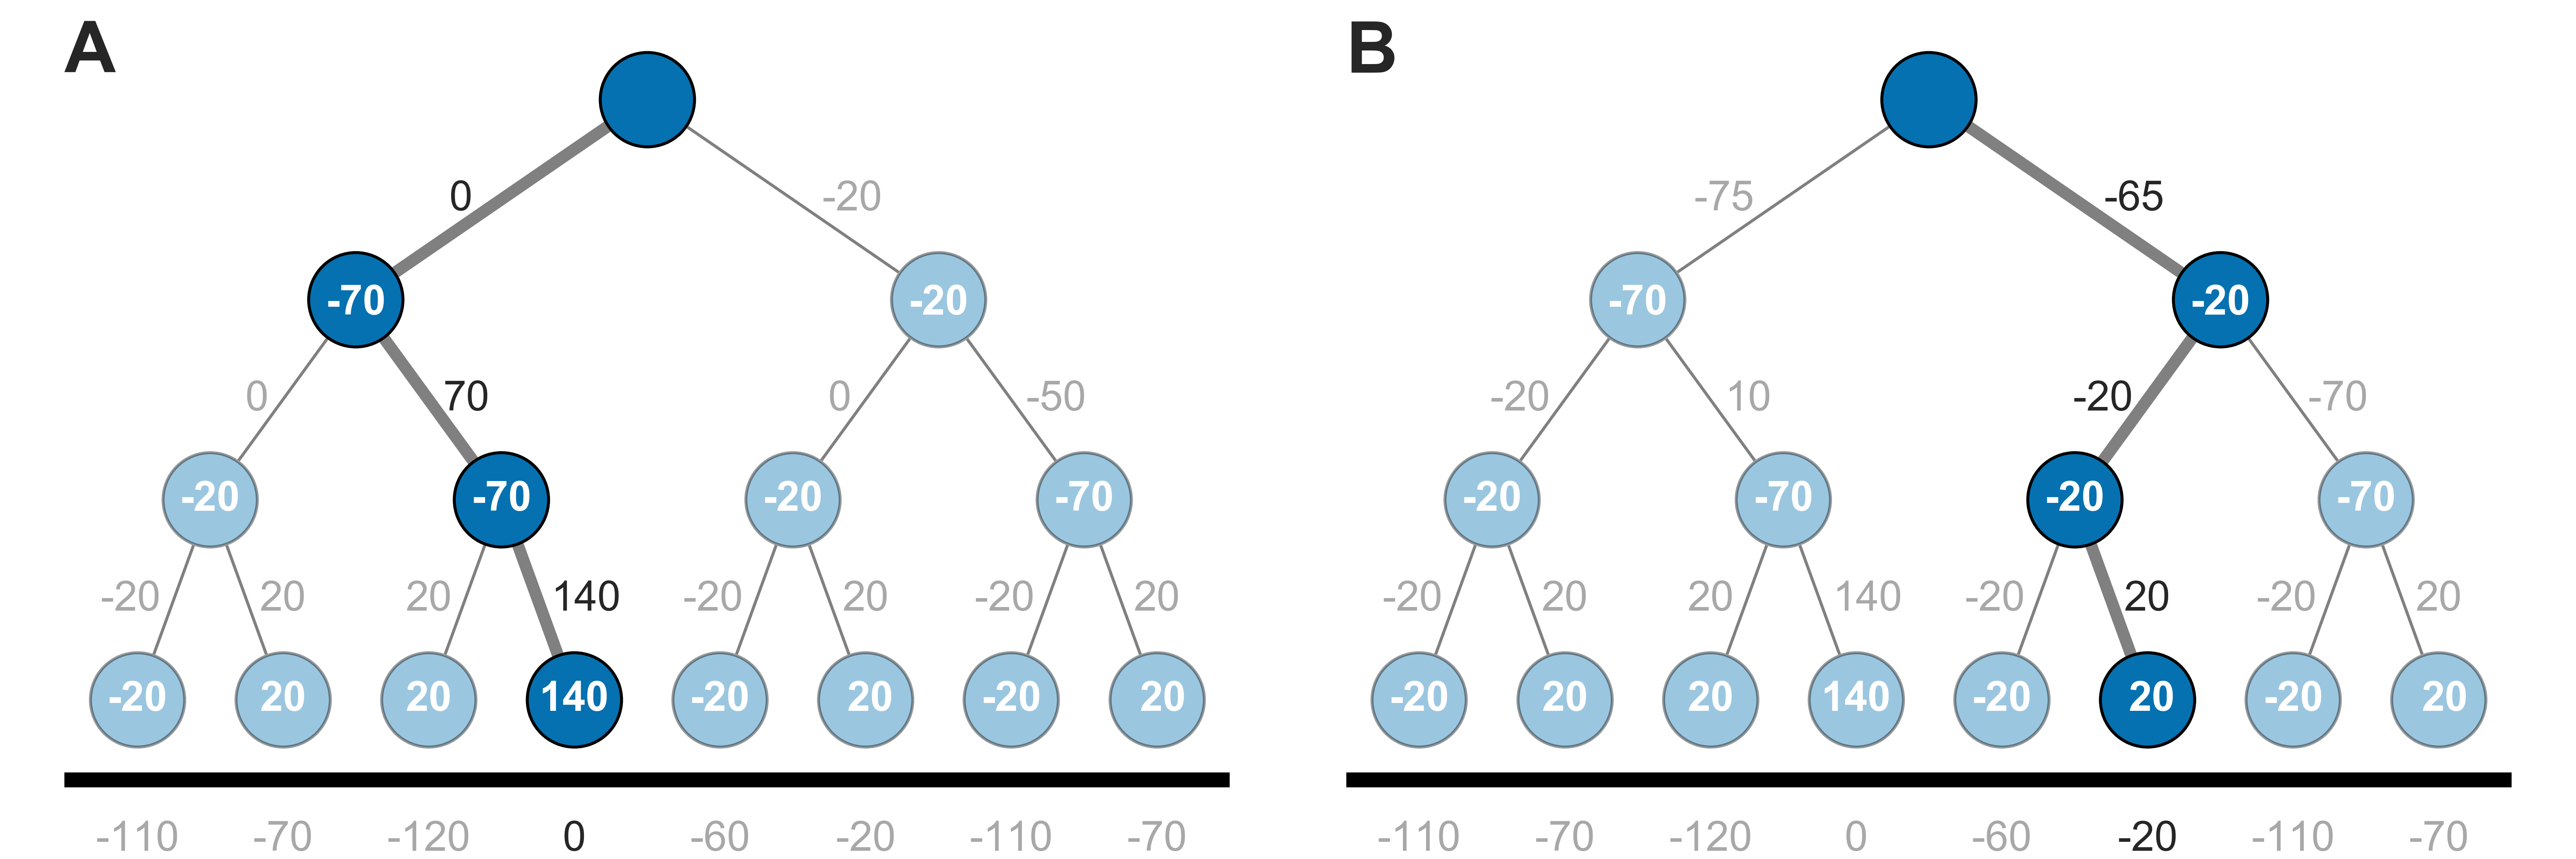
\includegraphics[trim={0 0 0 0},clip]{../figures/04_tree.png}}%
  }
  \caption{\textbf{Decision Tree}}
  \par remember to add parameters
\end{figure}

\subsection{Free Choice Premium}

If an agent is confident that their compentency in decision-making in intact,
then it follows that situations in which an individual is able to make a choice
should be preferable to situations in which an individual is not. At worst,
an agent is no better off than if they had not made a choice; at best, an agent
is better able to steer themselves toward desirable outcomes. Such is the logic
that underlies an increasingly robust literature suggesting choice is inherently
valuable \citep{Leotti2010}.

This free choice premium has been demonstrated multiple times in humans \citep{Suzuki1997,Leotti2011,Leotti2014,Cockburn2014} using a variety of decision
paradigms. For the present purposes, we will describe the experiments presented in
\citep{Leotti2011,Leotti2014}. In these experiments, participants complete a
two-stage decision making task (Figure 5). In the first stage, participants are
make a choice between two cues: one leading to free choice and the other leading
to a fixed choice. In the second stage, participants are able to choose between
a second set of cues (free choice) or are forced to choose a cue (fixed choice).
Unbeknownst to participants, all cues yield reward following the same outcome
distribution; thus, no cue is advantageous in the long-run. The free choice
premium is measured as a preference for the cue leading to free choice. \cite{Leotti2011,Leotti2014}
find participants still prefer the free choice cue, despite this conferring no
objective benefit to participants.

Insofar that this effect is contingent on the belief of one's own competency,
it stands to reason that this free choice premium should be absent in individuals
with anxiety and anxious control beliefs. We demonstrate this effect in Figure 5.
In each trial, the reward outcomes are equal for all options (-1, 1). In individuals
with increasingly pessimistic beliefs, the worst outcome in free choice is increasingly
back-propagated to the free-choice cue, thereby making it less attractive than
the fixed choice cue. Hence, pessimistic learners, on average, do not exhibit
this choice bias.

To our knowledge this prediction has not been empirically tested.

\begin{figure}
  \centerline{%
    \resizebox{1.0\textwidth}{!}{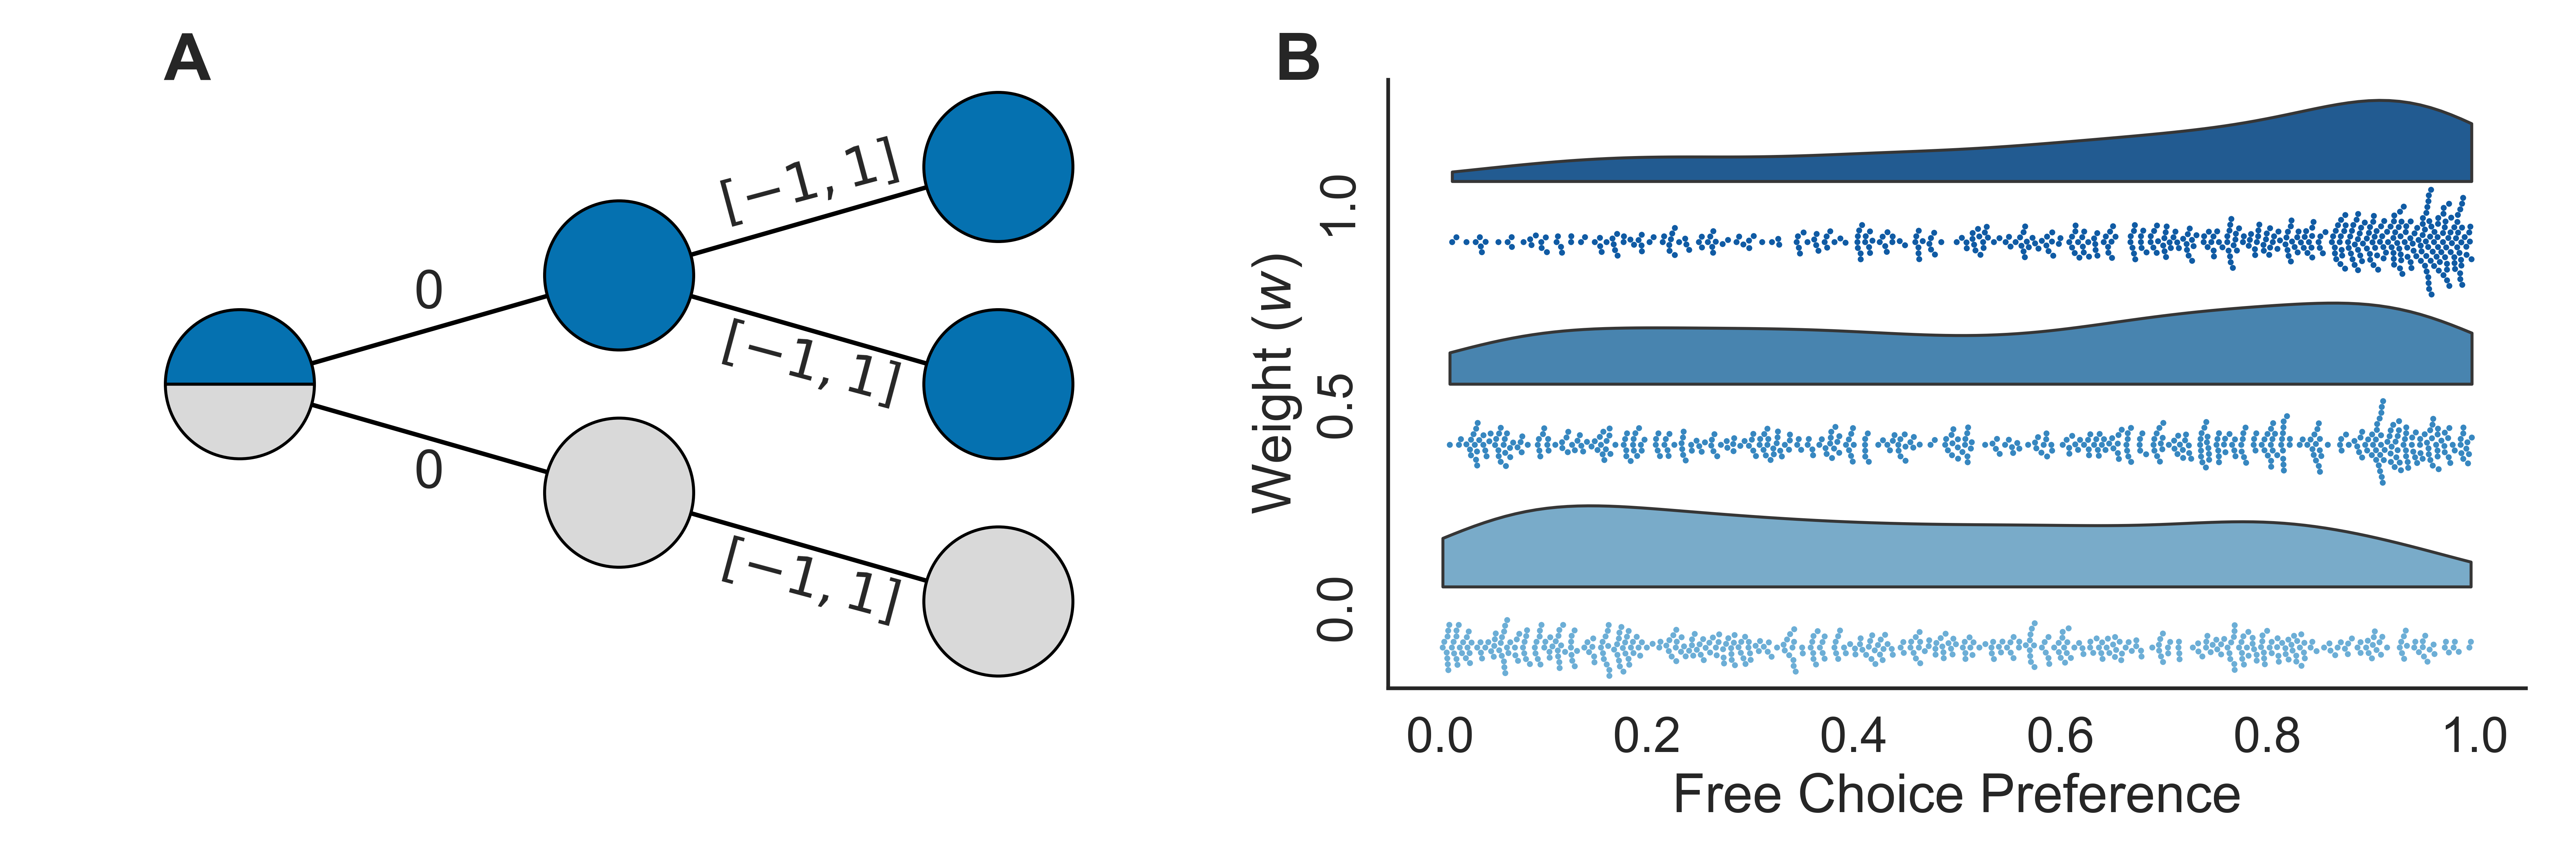
\includegraphics[trim={0 0 0 0},clip]{../figures/05_choice.png}}%
  }
  \caption{\textbf{Free Choice Premium}}
  \par remember to add parameters
\end{figure}

\subsection{Longitudinal Progression}

In this final section, we want to discuss the relationship between anxiety and
depression. Anxiety and depression are highly comorbid, with roughly 45% of individuals
with lifetime depression diagnosis also diagnosed with at least one anxiety disorder
\citep{kessler2015}. This fact has long been recognized in the clinical literature,
and prominent theories of depression have suggested that anxious control is a necessary
precursor to at least some types of depression \citep{alloy1990}. Recent large-scale
epidemiological studies have provided  some empirical support for this claim, finding that
anxiety symptoms precede and predict the onset of depression \citep{mathew2011, jacobson2014,
kessler2015} (though also see \cite{jacobson2017, plana2019}).

An emerging idea in this literature is that pathological avoidance as a result
of anxiety mediates the transition to depression, perhaps by reduce the likelihood
of experiencing positive events and activities \citep{moitra2008, jacobson2014}.
This finding is perfectly in line with the model presented so far. A sketch of
how this is possible is shown in Figure 6. Under unperturbed learning, avoidable
threat does not impede behavior. Under pessimistic learning, threat can block
future reward. This avoidance can manifest as a failure of behavioral initiation,
or a lack of overall mobility (here represented by an agent self-transitioning
at the starting state). Thus, the model can accomodate the deficits in positive
affect observed in depression as a function of behavioral avoidance, as predicted
by these epidemiological studies.

\begin{figure}
  \centerline{%
    \resizebox{1.0\textwidth}{!}{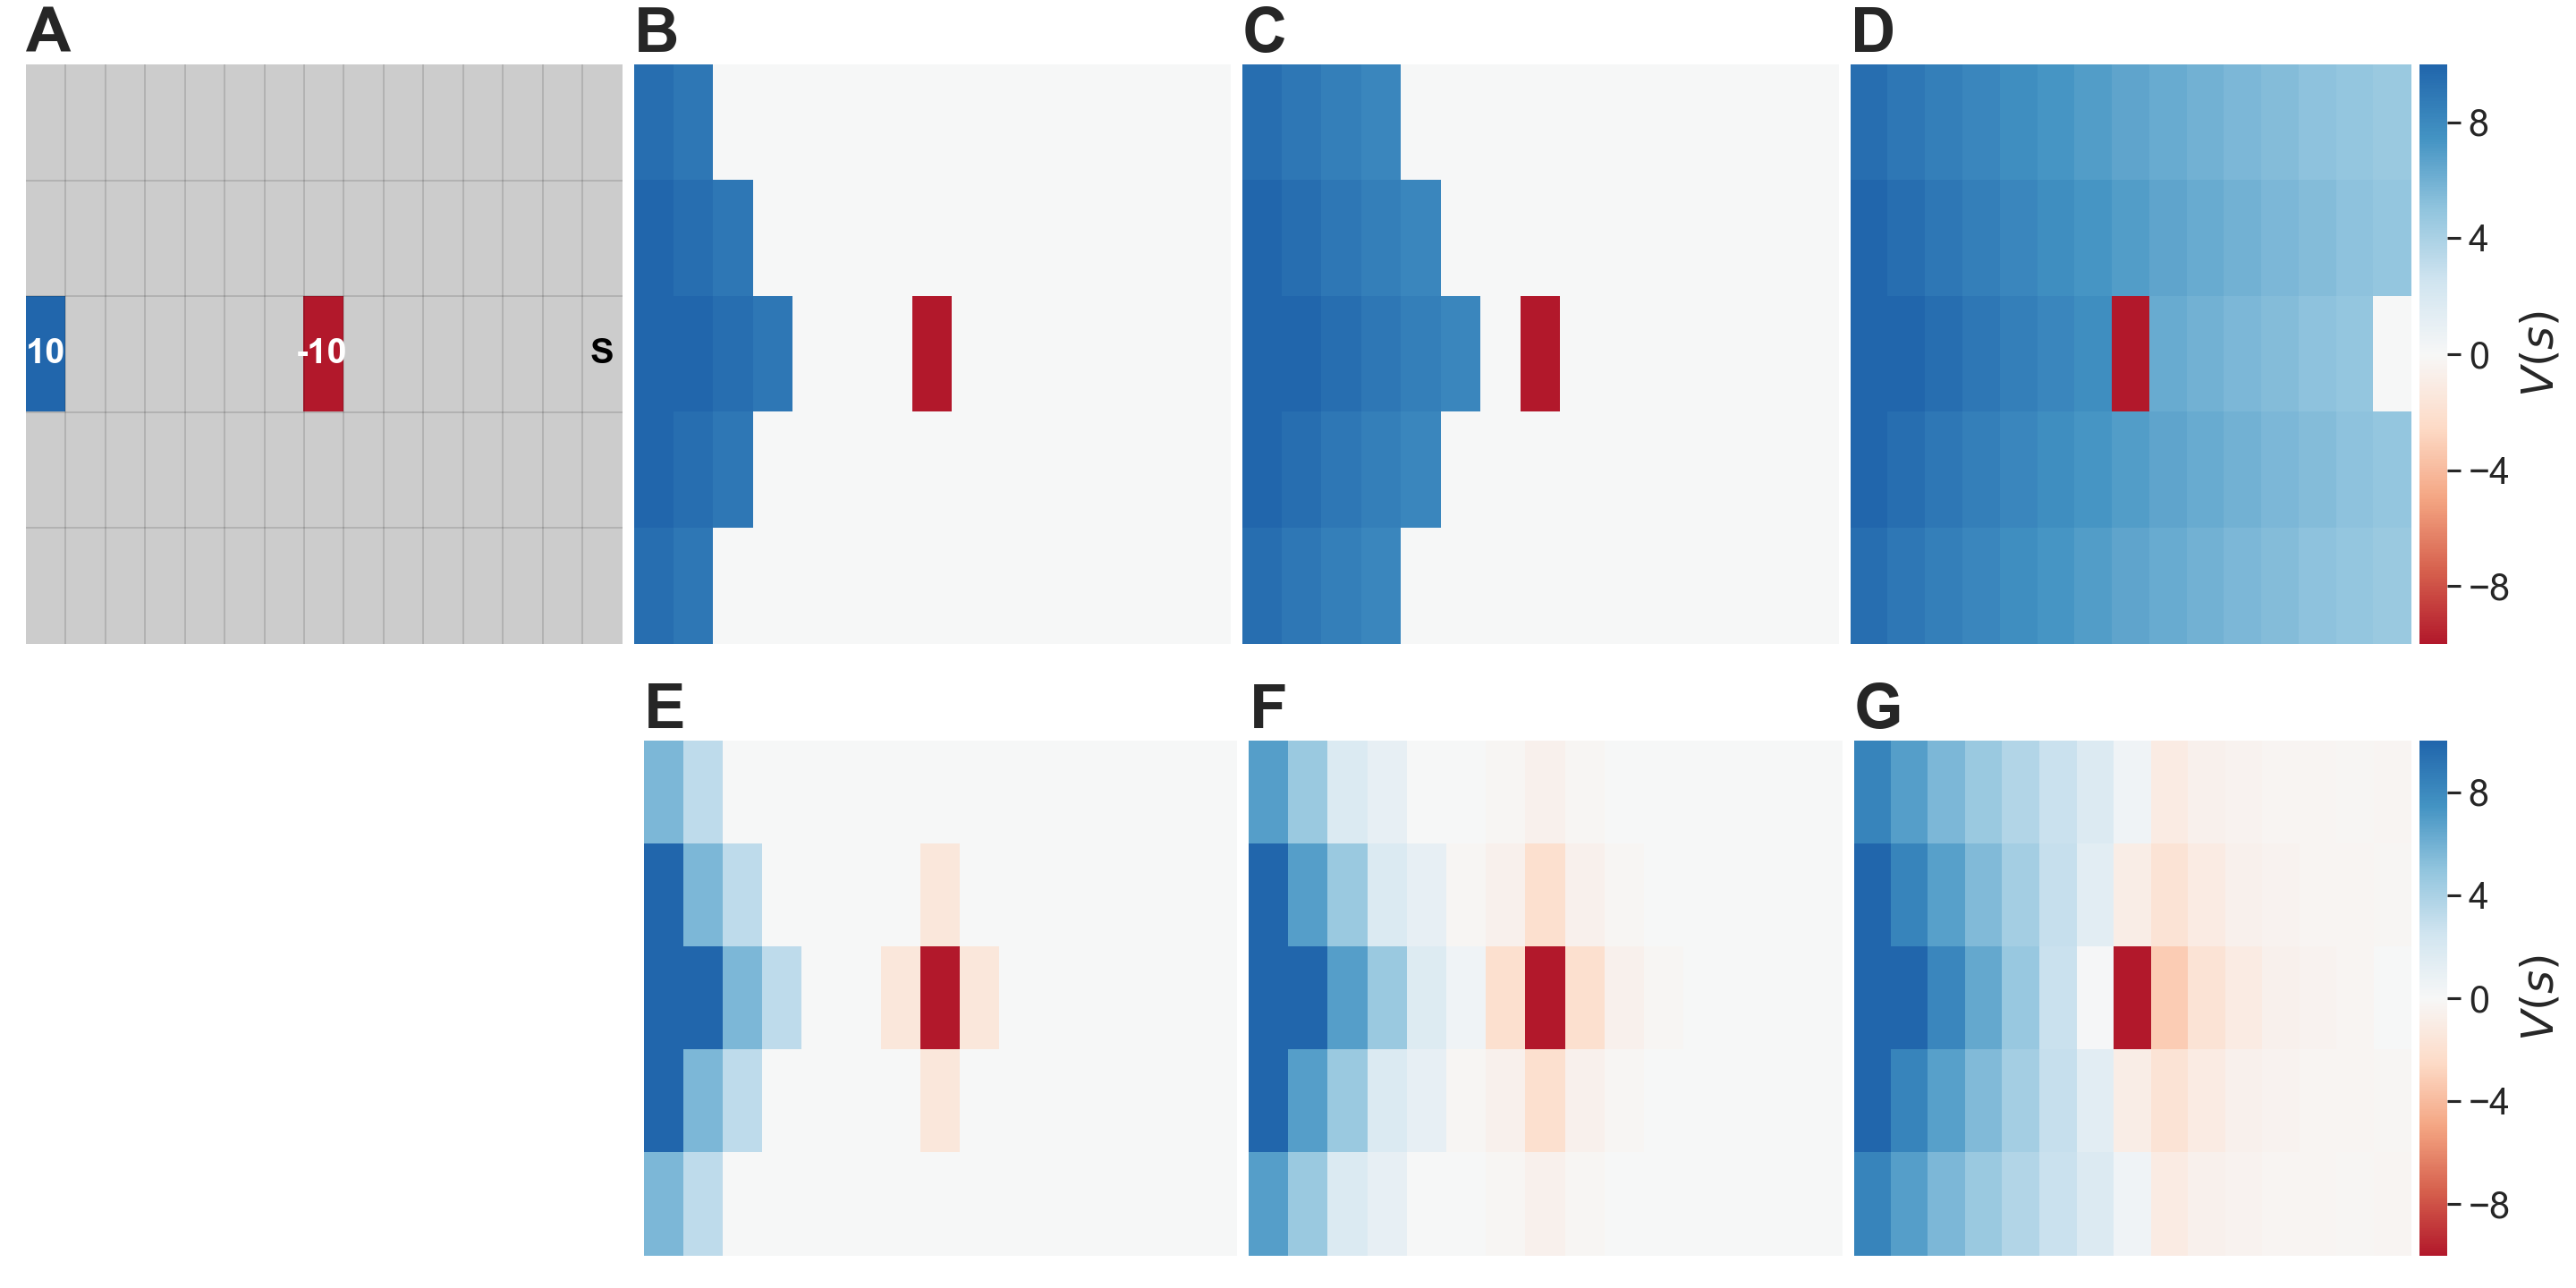
\includegraphics[trim={0 0 0 0},clip]{../figures/06_lh.png}}%
  }
  \caption{\textbf{Free Choice Premium}}
  \par remember to add parameters
\end{figure}

\section{Discussion}

In this article, we showed...

Discuss previous computational approaches: This has also been previously been
investigated in previous computational modeling \citep{HuysDayan2009}. There
the authors found that beliefs about a lack of controllability, mechanistically
modeled as corrupted priors about action-outcome contingencies, found deficient
learning in novel environments. The present results are no doubt related, but
address a different environment and a different behavior.

We discussed two mechanisms by which negative values can spread. There is a third
that we did not address here: that of the state itself. Here we assumed that states
were fully observable; in other words, there was no uncertainty about the state
an agent was currently occupying. In partially-observable Markov decision problems,
the state itself must be inferred from external and internal variables. This is
yet another means by which bad value can spread if undue likelihood is granted
to undesirable or aversive states. This ideas has previously been proposed to
explain some symptoms in anxiety \citep{Paulus2012}, and not without good reason.
Anxiety disorders involve negatively biased interpretation of ambiguous percepts
\citep{Hartley2012}, which may result in aberrant planning and increased avoidance
for similar reasons to those described above. This is an area for future research.

In this article, we have explored a computational principle of approach and
avoidance learning in sequential decision environments. We have not discussed,
however, the particular psychological or neurobiological mechanisms by which this
sort of learning may take place. This issue has been discussed in detail elsewhere
\citep{Bishop2018}, but we briefly discuss a few possibilities here. Mechanically,
we understand that complex decision problems are solved by mental processes that
exist on a spectrum between model-based and model-free (Daw et al., 2005). The
difference between these two families of methods hinges on the reliance of an
internal model of the world used to make predictions about expected long-run
outcomes of particular choices.

For model-based decision making, one possibility is biased planning. In large
state spaces, online sequential decision making suffers from the curve of
dimensionality: in planning a series of actions to take, comparing between
multiple options rapidly becomes computationally intractable when the number of
options and depth of search becomes even moderately large. Thus, heuristics for
reducing the size of this search can be useful. Biased pruning of search paths
(such as immediately discarding paths that require some minor loss in pursuit of
larger gains) may result in maladaptive decision making (Huys et al., 2012).
Alternately, if planning relies on internal sampling from previously experienced
episodes in order to make predictions about future value, then biased sampling
 may similarly result in maladaptive decision making. Recent work has shown how
 finite sampling during planning can result in risk aversion and the overrepresentation
 of low probability but strongly negative outcomes (Lieder et al., 2018). Such a
 mechanism is prima facie in line with results showing the availability in memory
 of negative outcomes being higher for patients with anxiety (Borkovec et al., 1999;
 Miranda and Mennin, 2007).

Within the realm of model-free decision making, several studies have found evidence
suggesting increased learning rates for negative reward prediction errors in
individuals with elevated levels of anxiety \citep{Aylward, Huang2017, Harle2017
garrett2018}. Though an asymmetry in sensitivity to
positive and negative reward prediction errors bears superficial similarity, for
the reasons described above merely attending more to negative information does not
necessarily predict increased avoidance insofar that avoidance can successfully
isolate negative outcomes. One possibility, and topic of future research, is how
prior beliefs about the reward statistics of the current environment dictate
learning rates. A second possibility is prioritized replay (Russek et al., 2017;
Mattar and Daw, 2018). Offline replay of previous experiences (through hippocampal
mechanisms) are known to facilitate learning. It has been proposed that biased
replay could bias value estimates (Gagne et al., 2018). This is another exciting
area for future research.


\section{References}

\bibliographystyle{vancouver-authoryear}
\bibliography{citations}

\section{Appendix}
\subsection{Algorithms}

\begin{algorithm}
  \caption{Value Iteration}

  \State Algorithm parameter: a small threshold $\theta > 0$ determining accuracy of estimation
  \State Initialize $V(s)$, for all $s \in S$ arbitrarily, except that $V(terminal) = 0$
  \State
  \While{$\Delta > \theta$}
    \State $\Delta \leftarrow 0$
    \Loop \ for each $s \in S$
      \State $v \leftarrow V(s)$
      \State $ V(s) = \max_a \sum_{s',r} p(s',r|s,a) \left[ r + \gamma V(s') \right] $
      \State $\Delta \leftarrow \max(\Delta, |v - V(s)|)$
    \EndLoop
  \EndWhile

\end{algorithm}

\begin{algorithm}
  \caption{Betamax Temporal Difference Learning}

  \State Algorithm parameters: step size $\eta \in (0, 1)$, small $\epsilon > 0$
  \State Initialize $Q(s,a)$, for all $s \in S$, $a \in A$ arbitrarily, except that $Q(terminal,\cdot) = 0$
  \State
  \Loop \ for each episode
    \State Initialize $S$
    \While{$S \notin S(terminal)$}
      \State Choose $A$ from $S$ using policy derived from $Q$
      \State Take action $A$, observe $R, S$
      \State $Q(S, A) \leftarrow Q(S, A) + \eta \left[ R + \gamma \max_a Q(S',a) − Q(S, A) \right] $
      \State $S \leftarrow S'$
    \EndWhile
  \EndLoop

\end{algorithm}

\end{document}
